% COMP3204 Coursework 2 -- CVPR format (max 4 pages of content + 1 page of references).
% Put this file next to the module's CVPR template files (cvpr.sty and the .bst file) and compile:
%   pdflatex report -> bibtex report -> pdflatex report -> pdflatex report
% Older CVPR kits use ieee_fullname.bst instead of ieeenat_fullname.bst (see \bibliographystyle below).
\documentclass[10pt,twocolumn,a4paper]{article}

\usepackage{cvpr}              % camera-ready; \usepackage[review]{cvpr} gives an anonymous draft
\usepackage{graphicx}
\usepackage{amsmath}
\usepackage{amssymb}
\usepackage{booktabs}
\usepackage[breaklinks,colorlinks,allcolors=blue]{hyperref}
\usepackage[capitalize]{cleveref}   % \cref / \Cref (load after hyperref)

\begin{document}

\title{What Makes a Style? Hand-Crafted Features versus a Foundation Model\\for 13-Class Painting Style Recognition}

\author{
Name Surname (ab1c23) \and Name Surname (ab1c23) \and Name Surname (ab1c23) \and Name Surname (ab1c23)\\
University of Southampton\\
{\tt\small \{ab1c23\}@soton.ac.uk}
}

\maketitle

% =====================================================================
\begin{abstract}
We classify 42{,}499 WikiArt paintings into 13 art movements. Our main system uses only techniques from the lectures: HSV colour histograms and statistics; Canny, Sobel, Gaussian scale-space and Fourier texture measures; Hough lines; Harris and Difference-of-Gaussian interest points; $k$-means regions with shape descriptors; and a bag of visual words built from DoG keypoints, our own gradient descriptors and $k$-means. With an RBF support vector machine it reaches 62.4\% accuracy and 0.610 macro-F1 on 8{,}500 held-out paintings (chance: 7.7\%). For every feature group we state the stylistic property it measures and the movements it separates, and support each claim with per-class feature statistics and a per-class permutation analysis. A frozen CLIP ViT-L/14 with an MLP head reaches 0.901 macro-F1 on the same split. Its advantage is largest on movements defined by subject matter rather than technique.
\end{abstract}

% =====================================================================
\section{Introduction}
\label{sec:intro}

An art movement combines \emph{technique} (palette, lighting, brushwork, composition) with \emph{content} (subjects, costume, era). Neighbouring movements often share technique, which makes style recognition a fine-grained problem. We ask how far classical computer vision can go on this problem, and which measurement is responsible for which decision. Our contributions are threefold.
\begin{enumerate}
\item A pipeline built from lecture techniques, each feature motivated by a stylistic property: colour spaces and histograms, Gaussian smoothing, Sobel and Canny edges, the Fourier transform, scale space, the Hough transform, Harris and DoG detectors, $k$-means segmentation, connected components, shape descriptors and PCA.
\item A per-class analysis that links each feature group to the movements it separates.
\item A foundation-model baseline (CLIP~\cite{radford2021learning}, self-study), evaluated on the identical test set.
\end{enumerate}

% =====================================================================
\section{Data and Problem}
\label{sec:data}

\begin{figure*}[t]
\centering
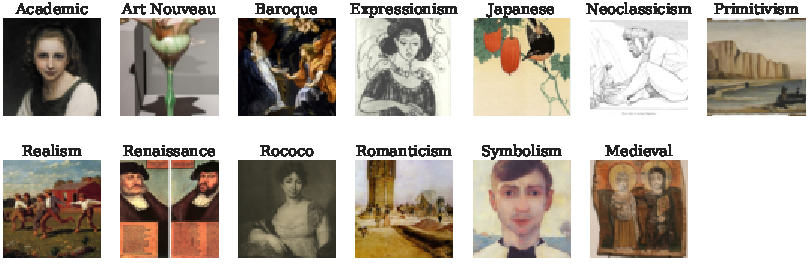
\includegraphics[width=\textwidth]{figures/examples.pdf}
\caption{One random painting per class (centre crop). The Neoclassicism example is an engraving: 47\% of that class is near-greyscale.}
\label{fig:examples}
\end{figure*}

We use the Kaggle \emph{WikiArt Art Movements/Styles} dataset~\cite{wikiart_kaggle}: 42{,}499 JPEG images in 13 classes (\cref{fig:examples}). The longer side of the images is 150--768 pixels. The classes are imbalanced by a factor of 5.9 (\cref{fig:counts}).

\begin{figure}[t]
\centering
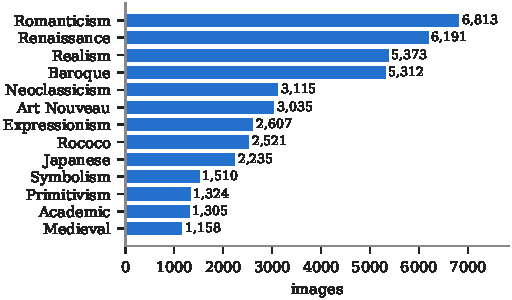
\includegraphics[width=0.82\columnwidth]{figures/class_counts.pdf}
\caption{Images per class.}
\label{fig:counts}
\end{figure}

\paragraph{Reflection.}
Four properties of the data shaped our design.
\begin{enumerate}
\item \textbf{Labels are historical movements, not visual categories.} Neoclassicism, Romanticism, Academic Art and Realism overlap in time (c.\ 1760--1900) and share oil technique, so some confusion is inherent.
\item \textbf{The medium differs between classes.} 9.6\% of all images are near-greyscale (mean saturation below 0.02), but the share is 47\% for Neoclassicism (engravings and drawings) and 0.1\% for Western Medieval. A classifier can therefore partly learn ``print'' instead of ``style''.
\item \textbf{Reproductions vary} in size, frame and exposure. We therefore normalise every feature for image size and crop the border first.
\item \textbf{There is no artist metadata.} The split is random and may share artists between training and test, which is known to inflate style accuracy~\cite{ashton2026style}. Both pipelines share the split, so the comparison between them remains fair.
\end{enumerate}

\paragraph{Protocol.}
A stratified 80/20 split (seed 42) gives 33{,}999 training and 8{,}500 test images. Every choice (hyper-parameters, vocabulary, scaling) is made by cross-validation on the training set, and each model sees the test set once. Because the classes are imbalanced, \textbf{macro-F1} is our main metric.

% =====================================================================
\section{Methods}
\label{sec:methods}

\begin{table*}[t]
\centering
\small
\begin{tabular}{@{}l r l l l@{}}
\toprule
Group & Dims & Techniques (lecture) & Stylistic property & Classes it helps most \\
\midrule
A1 colour histogram & 128 & HSV (CV10), joint $8{\times}4{\times}4$ histogram (L4, CV13) & palette & Primitivism, Medieval, Symbolism \\
A2 global colour stats & 15 & circular mean hue, $S$/$V$ moments and percentiles, colourfulness~\cite{hasler2003measuring} & lighting, saturation, format & Neoclassicism, Japanese, Art Nouveau \\
A3 colour grid & 54 & $H$/$S$/$V$ statistics in a $3{\times}3$ grid (CV13) & layout of light and colour & Neoclassicism, Medieval, Rococo \\
B edges \& texture & 34 & Gaussian (L5), Sobel (L6), Canny (L7), scale space (CV15), Fourier (L3) & brushwork, finish, detail & Japanese, Renaissance, Rococo \\
C lines & 5 & probabilistic Hough transform (L8) & straight, oriented structure & Medieval, Primitivism \\
D interest points & 8 & Harris corners, DoG blobs (CV15) & density and scale of detail & Medieval, Japanese \\
E regions & 6 & $k$-means, connected components (CV13); compactness, irregularity (CV14) & flat areas, fragmentation & Japanese, Art Nouveau \\
F visual words & 500 & DoG keypoints, Sobel descriptors, $k$-means vocabulary (CV15, L6, CV13) & vocabulary of local marks & Expressionism, Medieval, Academic \\
\bottomrule
\end{tabular}
\caption{The 750-dimensional traditional descriptor. L$n$ and CV$n$ refer to COMP3204 lectures~\cite{nixon2019feature}. The last column comes from \cref{fig:importance}.}
\label{tab:features}
\end{table*}

\paragraph{Pre-processing.}
Each image is prepared in three steps, with OpenCV~\cite{bradski2000opencv}:
\begin{enumerate}
\item The original aspect ratio is recorded, and 4\% is cropped from every side to remove frames and scan margins.
\item The image is resized so that its longer side is 512 pixels. Several features count events per pixel or depend on scale (edge density, Hough minimum line length, corner and blob densities), so a fixed scale makes them comparable. Area interpolation is used for shrinking and bilinear interpolation for the 2{,}725 enlarged images.
\item The image is converted to HSV (CV10), greyscale and Lab.
\end{enumerate}

\paragraph{Hand-crafted features (\cref{tab:features}).}
\begin{itemize}
\item \textbf{Colour (A).} The histogram gives most of its bins to hue, because HSV keeps a pigment in the same hue bin whatever its exposure.
\begin{itemize}
\item Hue is an angle, so its mean is a circular mean (sine and cosine), weighted by saturation so that grey pixels are ignored.
\item A2 adds the fractions of very dark ($V{<}0.2$), very bright ($V{>}0.8$) and strongly saturated pixels.
\item A3 repeats a reduced set of statistics per cell of a $3{\times}3$ grid, so that it records \emph{where} the light falls.
\end{itemize}
\item \textbf{Edges and texture (B).}
\begin{itemize}
\item Canny edges~\cite{canny1986computational}, with thresholds adapted to each image's median brightness after Gaussian smoothing, give edge density over the whole image and per grid cell.
\item Sobel gradients give an 8-bin orientation histogram (modulo $180^\circ$), weighted by magnitude.
\item Gradient statistics at $\sigma{=}1,2,4$ capture how fine detail vanishes at coarser scales.
\item The Fourier power of a Hann-windowed centre square is split into 6 frequency bands and 4 orientation sectors.
\end{itemize}
\item \textbf{Lines (C).} The probabilistic Hough transform~\cite{duda1972use,matas2000robust}, applied to the Canny map, gives line density, the straight fraction of the edges, and the horizontal, vertical and diagonal length shares.
\item \textbf{Interest points (D).} Harris~\cite{harris1988combined} gives corner density and strength. DoG~\cite{lowe2004distinctive} gives a histogram of blob sizes over 5 scales, a proxy for brush-stroke and detail scale. We use only OpenCV's SIFT \emph{detector}.
\item \textbf{Regions (E).} Lab colours are clustered by $k$-means ($k{=}8$, $k$-means++~\cite{arthur2007kmeans}), and each cluster is split into 8-connected components. We record the number of regions, the largest and median region area, the compactness and irregularity of the 10 largest regions, and the share of the dominant cluster.
\end{itemize}

\paragraph{Bag of visual words (F).}
Groups A--E summarise texture over the whole image, so they lose \emph{which kinds} of local marks a painter uses. Bag-of-words~\cite{csurka2004visual} is not covered in the lectures as a method, so we built it from lecture components in four steps:
\begin{enumerate}
\item \textbf{Keypoints.} The 600 strongest DoG keypoints are detected.
\item \textbf{Descriptors.} Each keypoint gets our own 128-value descriptor: Sobel orientation histograms over $4{\times}4$ cells of a patch whose radius follows the keypoint scale (8--32 pixels). The descriptor is L2-normalised, clipped at 0.2 and normalised again~\cite{lowe2004distinctive}.
\item \textbf{Vocabulary.} A 500-word vocabulary is learnt with $k$-means on 300{,}000 descriptors from 3{,}000 \emph{training} images.
\item \textbf{Encoding.} Each image becomes the normalised histogram of its nearest words.
\end{enumerate}
We also tested a $2{\times}2$ spatial pyramid~\cite{lazebnik2006beyond}.

\paragraph{Classifier.}
The features pass through three steps before classification.
\begin{enumerate}
\item The histogram groups (A1, F) are square-rooted (Hellinger mapping).
\item All features are standardised.
\item Each group is scaled by $1/\sqrt{d_g}$, where $d_g$ is its dimension, so that every group carries equal variance and 500 visual words cannot drown out 5 line features.
\end{enumerate}
An RBF SVM~\cite{cortes1995support} ($\gamma=1/(d\,\mathrm{Var}\,X)$) is tuned over $C\in\{3,10,30\}$ by 3-fold stratified cross-validation on macro-F1; $C{=}10$ is selected. $k$-NN (with optional PCA, CV12) and a random forest are baselines tuned in the same way. Every fitted step sits inside the cross-validation pipeline~\cite{pedregosa2011scikit}.

\paragraph{Deep baseline (self-study).}
We use a frozen CLIP ViT-L/14~\cite{radford2021learning,dosovitskiy2021image} pre-trained on DataComp-XL~\cite{gadre2023datacomp}.
\begin{itemize}
\item \textbf{Input.} Each painting is embedded as one $224^2$ global view plus the mean of four $224^2$ tiles from a $448^2$ resize, which adds brushwork detail.
\item \textbf{Head.} A two-layer MLP (1{,}024 units, GELU, dropout) is trained with class-weighted, label-smoothed cross-entropy. It stops early on the validation macro-F1 of a 12.5\% split of the training set.
\item \textbf{Alternatives.} DINOv2 ViT-L/14~\cite{oquab2024dinov2} alone (0.819) and combined with CLIP (0.900) were worse on validation than CLIP alone (0.903).
\end{itemize}

% =====================================================================
\section{Validation and Results}
\label{sec:results}

\begin{table}[t]
\centering
\small
\begin{tabular}{@{}l c c@{}}
\toprule
Model (13 classes, test set) & Acc.\ (\%) & Macro-F1 \\
\midrule
$k$-NN, groups A--E & 47.6 & 0.439 \\
Random forest, groups A--E & 53.3 & 0.484 \\
SVM, groups A--E & 58.9 & 0.571 \\
\quad + visual words, $K{=}200$ & 61.6 & 0.596 \\
\quad + visual words, $K{=}500$ \textbf{(final)} & \textbf{62.4} & \textbf{0.610} \\
\quad + $2{\times}2$ spatial pyramid & 62.9 & 0.612 \\
\midrule
CLIP ViT-L/14 + MLP (deep) & 90.4 & 0.901 \\
\bottomrule
\end{tabular}
\caption{Test results. Each indented row adds one component to the row above it. The pyramid gains 0.002 for $4\times$ the training time, so it is not used.}
\label{tab:results}
\end{table}

\begin{table}[t]
\centering
\small
\begin{tabular}{@{}l r c c c@{}}
\toprule
Class & Test $n$ & Ours & CLIP & Gap \\
\midrule
Japanese Art & 447 & 0.772 & 0.968 & 0.20 \\
Neoclassicism & 623 & 0.728 & 0.884 & 0.16 \\
Western Medieval & 232 & 0.719 & 0.968 & 0.25 \\
Renaissance & 1238 & 0.662 & 0.948 & 0.29 \\
Primitivism & 265 & 0.656 & 0.968 & 0.31 \\
Art Nouveau & 607 & 0.646 & 0.927 & 0.28 \\
Realism & 1075 & 0.620 & 0.897 & 0.28 \\
Expressionism & 521 & 0.615 & 0.939 & 0.32 \\
Baroque & 1062 & 0.613 & 0.908 & 0.30 \\
Romanticism & 1363 & 0.609 & 0.877 & 0.27 \\
Rococo & 504 & 0.489 & 0.854 & 0.37 \\
Academic Art & 261 & 0.416 & 0.788 & 0.37 \\
Symbolism & 302 & 0.380 & 0.791 & 0.41 \\
\midrule
Macro average & 8500 & 0.610 & 0.901 & 0.29 \\
\bottomrule
\end{tabular}
\caption{Per-class test F1 of our final model and of CLIP.}
\label{tab:perclass}
\end{table}

\begin{figure}[t]
\centering
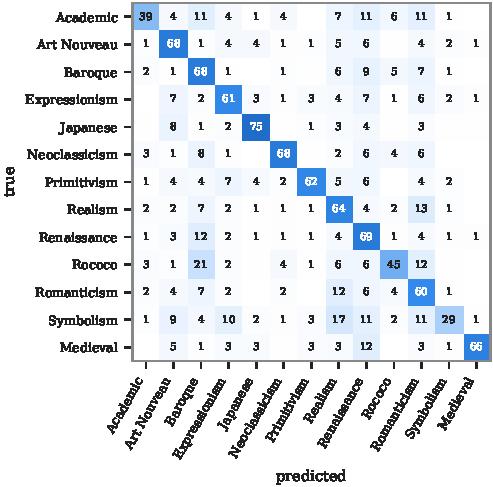
\includegraphics[width=\columnwidth]{figures/confusion.pdf}
\caption{Row-normalised test confusion matrix (\%) of our final model.}
\label{fig:confusion}
\end{figure}

\paragraph{Overall.}
\Cref{tab:results} shows three results.
\begin{itemize}
\item On the same features, the SVM clearly beats $k$-NN and the random forest.
\item Visual words add 3.9 macro-F1 points, and a larger vocabulary helps further.
\item The spatial pyramid does not help: \emph{which} marks a painter uses matters more than \emph{where} they occur.
\end{itemize}
The final model scores 0.575 in cross-validation, where each fold trains on two-thirds of the data, and 0.610 on the test set, about 8 times chance.

\paragraph{Per class.}
The strongest classes are Japanese Art, Neoclassicism and Western Medieval (\cref{tab:perclass}). Each has a distinctive \emph{look}: flat colour on light paper, monochrome prints, and saturated outlined panels respectively. The errors follow art history (\cref{fig:confusion}):
\begin{itemize}
\item Rococo is predicted as Baroque in 21\% of cases;
\item Symbolism as Realism in 17\%;
\item Realism and Romanticism are confused in 12--13\% of cases each way;
\item Medieval is predicted as Renaissance, and Renaissance as Baroque, in 12\% of cases each.
\end{itemize}
CLIP's most confused validation pairs (Neoclassicism--Rococo, Realism--Romanticism, Baroque--Rococo) overlap with ours, which points to genuine ambiguity in the labels.

\paragraph{Leakage check.} 161 test images are near-duplicates of a training image (DINOv2 cosine $>0.97$). Removing them changes CLIP's macro-F1 only from 0.901 to 0.899.

% =====================================================================
\section{Discussion: Which Feature Separates Which Style}
\label{sec:discussion}

\begin{figure}[t]
\centering
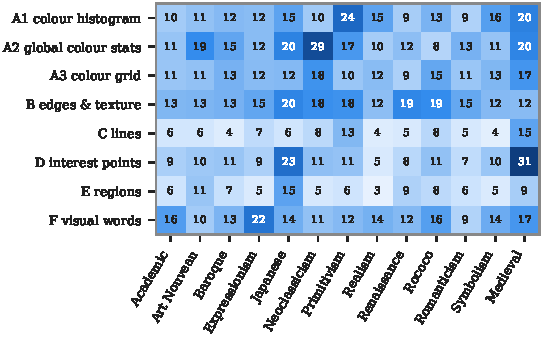
\includegraphics[width=\columnwidth]{figures/group_importance.pdf}
\caption{Drop in per-class test F1 ($\times 100$) when one feature group is shuffled across test images (mean of 2 repeats). Read across a row: the classes with the largest drops rely most on that group.}
\label{fig:importance}
\end{figure}

We shuffle one group's columns across the test images and record the drop in each class's F1 (\cref{fig:importance}). Any shuffle adds noise to every RBF distance, so all classes drop. The informative part is how a group's drop \emph{varies across classes}. Below, each group's largest drops are given in brackets, explained using class means of the features.

\paragraph{A1 Colour histogram: Primitivism (24), Medieval (20), Symbolism (16).}
\begin{itemize}
\item \textbf{Primitivism and Medieval} are the most saturated movements. 35\% and 37\% of their pixels are strongly saturated (overall: 23\%), and their colourfulness is 0.22 and 0.20 (overall: 0.14): naive flat colour, and gold, vermilion and ultramarine tempera. They are recognised by \emph{which} hues appear.
\item \textbf{Symbolism} has no distinctive texture or lighting, so its palette is its best cue.
\end{itemize}

\paragraph{A2 Global statistics: Neoclassicism (29), Japanese (20), Art Nouveau (19).}
\begin{itemize}
\item \textbf{Neoclassicism} is the least colourful class (0.08), because half of it is greyscale prints.
\item \textbf{Japanese and Art Nouveau} have the most very bright pixels (35\% and 37\%, against 20\%) from paper and light poster grounds, but few saturated ones (13--15\%).
\item \textbf{Baroque} (15) has the most very dark pixels (31\%, against 18\%): its tenebrism.
\end{itemize}

\paragraph{A3 Colour grid: Neoclassicism (18), Medieval (17), Rococo (15).}
\begin{itemize}
\item \textbf{Rococo} shows by far the strongest bright-centre, dark-corner pattern ($+0.15$ in $V$, against $+0.03$): a lit sitter against a darkened ground. Baroque follows ($+0.08$).
\item \textbf{Realism and Romanticism} have the brightest top rows ($+0.12$ and $+0.10$ top minus bottom, against $+0.06$): sky above land.
\end{itemize}

\paragraph{B Edges and texture: Japanese (20), Renaissance (19), Rococo (19).}
This group separates opposite finishes.
\begin{itemize}
\item \textbf{Smooth: Rococo and Academic.} They have the lowest edge density (6.8\% and 5.9\%, against 7.9\%) and the lowest high-frequency power (6.0\% and 5.7\%, against 9.6\%): blended, invisible brushwork.
\item \textbf{Linear and ornamental: Medieval, Art Nouveau, Japanese and Neoclassical images} carry the most high-frequency power (12.0--14.2\%), from outlines, ornament and hatching.
\item \textbf{Crisp: Renaissance} has the highest edge density of the oil-painting classes (9.6\%): sharp contours and fine detail.
\end{itemize}

\paragraph{C Lines: Medieval (15), Primitivism (13).}
\begin{itemize}
\item \textbf{Medieval} has the most straight lines (8.8 against 6.0 per $10^4$ pixels) and the most vertical ones (37\% of line length, against 25\%): frames, thrones, architecture.
\item \textbf{Primitivism}, like Realism and Romanticism, favours horizontals (33\%): horizons.
\item \textbf{Baroque and Rococo} have the most diagonals (58\% and 61\%, against 50\%), matching their dynamic compositions, but this cue is weak (4--8 points).
\end{itemize}

\paragraph{D Interest points: Medieval (31), Japanese (23).}
\begin{itemize}
\item \textbf{Medieval} has 104 Harris corners and 110 small DoG blobs per $10^4$ pixels (averages: 66 and 64), from haloes, ornament, punched gold and script.
\item \textbf{Japanese prints} have 87 corners and 77 small blobs, from patterned fabric and linework.
\item \textbf{Rococo and Academic} have the fewest: about 38 corners and 43 small blobs.
\end{itemize}

\paragraph{E Regions: Japanese (15), Art Nouveau (11).}
\begin{itemize}
\item \textbf{Japanese and Art Nouveau} have the largest single region (21\% of the image, against 17\%): flat backgrounds.
\item \textbf{Renaissance and Medieval} split into the most regions (136 and 132, against 111).
\end{itemize}

\paragraph{F Visual words: Expressionism (22), Medieval (17), Academic (16).}
Expressionism is close to average on every global statistic: 7.1\% edges against 7.9\%, and 9.7\% high-frequency power against 9.6\%. What sets it apart is the \emph{type} of mark (bold strokes, thick outlines), which only a vocabulary of local descriptors captures. This explains the 3.9-point gain from visual words.

\paragraph{Why the hardest classes fail.}
Rococo, Academic Art and Symbolism are defined largely by content, and their low-level statistics overlap with those of their neighbours.
\begin{itemize}
\item \textbf{Rococo} is usually described as pastel, but here it is \emph{dark}. 27\% of its pixels are very dark (Baroque: 31\%), and it has the fewest bright pixels of any class (9\%). What separates it from Baroque is subject and costume, which our features cannot see. This explains the 21\% Rococo$\rightarrow$Baroque error.
\item \textbf{Academic Art} shares Rococo's smooth finish and Romanticism's subjects.
\item \textbf{Symbolism} has no low-level signature at all.
\end{itemize}
These are the classes where CLIP gains most ($+0.37$ to $+0.41$), as it recognises objects, clothing and scene types learnt from billions of image--text pairs. Its smallest gains, on Neoclassicism ($+0.16$) and Japanese Art ($+0.20$), are where low-level cues already suffice.

\paragraph{Context and limitations.}
On the full 25--27-style WikiArt task, published results range from 46\% with hand-crafted features and metric learning~\cite{saleh2016large} to 54--63\% with fine-tuned CNNs~\cite{tan2016ceci,lecoutre2017recognizing}. These numbers are not directly comparable with ours, because those tasks have more and finer classes. Our results have three limitations:
\begin{itemize}
\item Artists may be shared between training and test~\cite{ashton2026style}.
\item CLIP may have seen WikiArt during pre-training.
\item Part of the Neoclassicism score reflects the print medium rather than the style.
\end{itemize}

% =====================================================================
\section{Conclusion}
Lecture techniques, each tied to a concrete property of painting style, reach 0.610 macro-F1 on 13 movements, and the evidence shows when they work:
\begin{itemize}
\item colour statistics separate greyscale prints, light Japanese and Art Nouveau works, and saturated Medieval and Primitivist works;
\item edge, texture and interest-point features separate the smooth Academic and Rococo finish from detailed Medieval, Renaissance and Japanese work;
\item lines and regions capture vertical and flat compositions;
\item visual words capture Expressionist brushwork.
\end{itemize}
Movements defined by content remain out of reach for low-level features. A frozen foundation model closes most of the gap (0.901): beyond about 0.6 macro-F1, painting style becomes a semantic problem.

\paragraph{Individual contributions.}
% TODO: replace with the team's real contributions.
\emph{Name 1}: \dots\ \emph{Name 2}: \dots\ \emph{Name 3}: \dots\ \emph{Name 4}: \dots

{\small
\bibliographystyle{ieeenat_fullname}
\bibliography{references}
}

\end{document}
